\documentclass[../../main/main.tex]{subfiles}
\graphicspath{{./figures/}}

\dominitoc
\faketableofcontents

% \renewcommand{\mtcSfont}{\small\bfseries}
% \renewcommand{\mtcSSfont}{\footnotesize}
\mtcsettitle{minitoc}{}
\mtcsetrules{*}{off}

\makeatletter
\renewcommand{\@chapapp}{\'Electrocin\'etique -- chapitre}
\renewcommand{\chaplett}{E}
\makeatother

% \toggletrue{student}
% \toggletrue{corrige}
% \renewcommand{\mycol}{black}
% \renewcommand{\mycol}{gray}

\hfuzz=5.003pt

\begin{document}
\setcounter{chapter}{2}

\settype{book}
\settype{prof}
\settype{stud}

\chapter{Circuits du 1\ier{} ordre}

\vspace*{\fill}

\begin{tcn}(appl)<ctc>"somm"'t'{Sommaire}
	\let\item\olditem
	\vspace{-15pt}
	\minitoc
	\vspace{-25pt}
\end{tcn}

\begin{tcn}[sidebyside](appl)<ctb>"how"'t'{Capacités exigibles}
	\begin{itemize}[label=\rcheck]
			\item Distinguer, sur un relevé expérimental, régime transitoire et
			      régime permanent au cours de l'évolution d'un système du premier
			      ordre soumis à un échelon de tension.
			\item Interpréter et utiliser la continuité de la tension aux bornes d'un
			      condensateur ou de l'intensité du courant traversant une bobine.
			\item Réaliser un bilan énergétique.
	\end{itemize}
	\tcblower
	\begin{itemize}[label=\rcheck]
			\item Établir l'équation différentielle du premier ordre vérifiée par une
			      grandeur électrique dans un circuit comportant une ou deux mailles.
			\item Déterminer la réponse temporelle dans le cas d'un régime libre ou
			      d'un échelon de tension
			\item Déterminer un ordre de grandeur de la durée du régime transitoire.
	\end{itemize}
\end{tcn}

\vspace*{\fill}
\newpage
\vspace*{\fill}

%\vspace{-15pt}
\begin{tcn}[%
		sidebyside, fontupper=\small, fontlower=\small
	](appl)<ctb>"chek"'t'{L'essentiel}
	\begin{tcn}[nsp](defi)<ctc>'t'{Définitions}
		\tcblistof[\paragraph*]{defi}{\hspace*{4.8pt}}
	\end{tcn}
	% \begin{tcn}[nsp](rapp)<ctc>'t'{Rappels}
	% 	\tcblistof[\paragraph*]{rapp}{\hspace*{4.8pt}}
	% \end{tcn}
	\begin{tcn}[nsp](prop)<ctc>'t'{Propriétés}
		\tcblistof[\paragraph*]{prop}{\hspace*{4.8pt}}
		% \tcblistof[\paragraph*]{loi}{\hspace*{4.8pt}}
		% \tcblistof[\paragraph*]{theo}{\hspace*{4.8pt}}
	\end{tcn}
	% \begin{tcn}[nsp](loi)<ctc>'t'{Lois}
	% 	\tcblistof[\paragraph*]{loi}{\hspace*{4.8pt}}
	% \end{tcn}
	% \begin{tcn}[nsp](coro)<ctc>'t'{Corollaires}
	%   \tcblistof[\paragraph*]{coro}{\hspace*{4.8pt}}
	% \end{tcn}
	% \begin{tcn}[nsp](demo)<ctc>'t'{Démonstrations}
	% 	\tcblistof[\paragraph*]{demo}{\hspace*{4.8pt}}
	% 	\tcblistof[\paragraph*]{prev}{\hspace*{4.8pt}}
	% \end{tcn}
	% \begin{tcn}[nsp](inte)<ctc>'t'{Interprétations}
	% 	\tcblistof[\paragraph*]{inte}{\hspace*{4.8pt}}
	% \end{tcn}
	\begin{tcn}[nsp](impl)<ctc>'t'{Implications}
		\tcblistof[\paragraph*]{impl}{\hspace*{4.8pt}}
	\end{tcn}
	% \begin{tcn}[nsp](tool)<ctc>'t'{Outils}
	% 	\tcblistof[\paragraph*]{tool}{\hspace*{4.8pt}}
	% \end{tcn}
	% \begin{tcn}[nsp](nota)<ctc>'t'{Notations}
	% 	\tcblistof[\paragraph*]{nota}{\hspace*{4.8pt}}
	% \end{tcn}
	% \begin{tcn}[nsp](appl)<ctc>'t'{Applications}
	% 	\tcblistof[\paragraph*]{appl}{\hspace*{4.8pt}}
	% \end{tcn}
	% \begin{tcn}[nsp](rema)<ctc>'t'{Remarques}
	%   \tcblistof[\paragraph*]{rema}{\hspace*{4.8pt}}
	% \end{tcn}
	% \begin{tcn}[nsp](exem)<ctc>'t'{Exemples}
	%   \tcblistof[\paragraph*]{exem}{\hspace*{4.8pt}}
	% \end{tcn}
	% \begin{tcn}[nsp](ror)<ctc>"hart"'t'{Points importants}
	%   \tcblistof[\paragraph*]{ror}{\hspace*{4.8pt}}
	% \end{tcn}
	% \begin{tcn}[nsp](impo)<ctc>'t'{Erreurs communes}
	%   \tcblistof[\paragraph*]{impo}{\hspace*{4.8pt}}
	% \end{tcn}
	\tcblower
	% \begin{tcn}[nsp](defi)<ctc>'t'{Définitions}
	%   \tcblistof[\paragraph*]{defi}{\hspace*{4.8pt}}
	% \end{tcn}
	% \begin{tcn}[nsp](rapp)<ctc>'t'{Rappels}
	%   \tcblistof[\paragraph*]{rapp}{\hspace*{4.8pt}}
	% \end{tcn}
	% \begin{tcn}[nsp](prop)<ctc>'t'{Propriétés}
	% \tcblistof[\paragraph*]{prop}{\hspace*{4.8pt}}
	% \tcblistof[\paragraph*]{loi}{\hspace*{4.8pt}}
	% \tcblistof[\paragraph*]{theo}{\hspace*{4.8pt}}
	% \end{tcn}
	% \begin{tcn}[nsp](coro)<ctc>'t'{Corollaires}
	%   \tcblistof[\paragraph*]{coro}{\hspace*{4.8pt}}
	% \end{tcn}
	\begin{tcn}[nsp](demo)<ctc>'t'{Démonstrations}
		\tcblistof[\paragraph*]{demo}{\hspace*{4.8pt}}
		% \tcblistof[\paragraph*]{prev}{\hspace*{4.8pt}}
	\end{tcn}
	% \begin{tcn}[nsp](inte)<ctc>'t'{Interprétations}
	% 	\tcblistof[\paragraph*]{inte}{\hspace*{4.8pt}}
	% \end{tcn}
	% \begin{tcn}[nsp](impl)<ctc>'t'{Implications}
	% 	\tcblistof[\paragraph*]{impl}{\hspace*{4.8pt}}
	% \end{tcn}
	% \begin{tcn}[nsp](tool)<ctc>'t'{Outils}
	%   \tcblistof[\paragraph*]{tool}{\hspace*{4.8pt}}
	% \end{tcn}
	% \begin{tcn}[nsp](nota)<ctc>'t'{Notations}
	% 	\tcblistof[\paragraph*]{nota}{\hspace*{4.8pt}}
	% \end{tcn}
	% \begin{tcn}[nsp](odgr)<ctc>'t'{Ordres de grandeur}
	% 	\tcblistof[\paragraph*]{odgr}{\hspace*{4.8pt}}
	% \end{tcn}
	% \begin{tcn}[nsp](appl)<ctc>'t'{Applications}
	% 	\tcblistof[\paragraph*]{appl}{\hspace*{4.8pt}}
	% \end{tcn}
	% \begin{tcn}[nsp](rema)<ctc>'t'{Remarques}
	%   \tcblistof[\paragraph*]{rema}{\hspace*{4.8pt}}
	% \end{tcn}
	% \begin{tcn}[nsp](exem)<ctc>'t'{Exemples}
	% 	\tcblistof[\paragraph*]{exem}{\hspace*{4.8pt}}
	% \end{tcn}
	\begin{tcn}[nsp](ror)<ctc>"hart"'t'{Points importants}
		\tcblistof[\paragraph*]{ror}{\hspace*{4.8pt}}
	\end{tcn}
	\begin{tcn}[nsp](impo)<ctc>'t'{Erreurs communes}
		\tcblistof[\paragraph*]{impo}{\hspace*{4.8pt}}
	\end{tcn}
\end{tcn}

\vspace*{\fill}

On appelle \textbf{circuit linéaire du premier ordre} un circuit électrique
dont l'évolution des grandeurs électriques est régie par des équations
différentielles linéaires à coefficients constants et \textit{du premier
	ordre}. On étudie ici leur réponse à un échelon de tension.

\vspace*{\fill}

\newpage

\section{Circuit RC}
\subsection{Circuit RC série~: charge}

\begin{tcb}[label=def:echelon, sidebyside, righthand ratio=.25]
  (defi){Échelon de tension}
	Un échelon de tension est montant s'il est de la forme
	\[
		\left\{
		\begin{array}{rcl}
			u(t<0)    & = & 0 \\
			u(t\geq0) & = & E
		\end{array}
		\right.
	\]
	et descendant si $E$ avant et 0 après.
	\tcblower
	\begin{center}
		\sswitch{%
			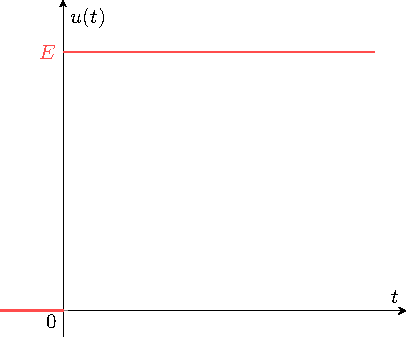
\includegraphics[width=\linewidth, draft=true]{echelon}
		}{%
			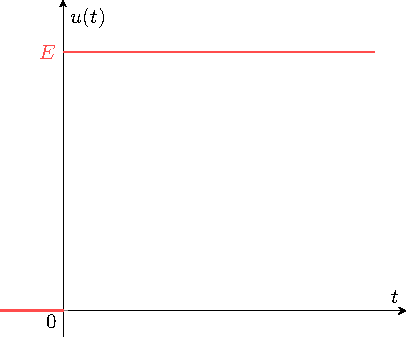
\includegraphics[width=\linewidth]{echelon}
		}%
		\captionof{figure}{}
	\end{center}
\end{tcb}

\subsubsection{Présentation}
\begin{tcb*}[sidebyside, righthand ratio=.30](defi){Circuit RC en charge}
  \begin{itemize}
    \item Il est constitué d'un générateur idéal de tension en série avec une
          résistance et un condensateur idéal.
    \item \textbf{On suppose le condensateur initialement déchargé}.
    \item À $t=0$, on ferme l'interrupteur.
  \end{itemize}
\tcblower
  \begin{center}
    \sswitch{%
      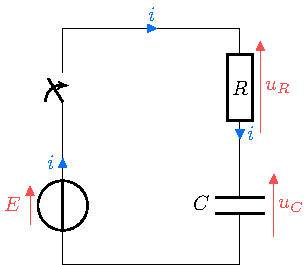
\includegraphics[width=.9\linewidth, draft=true]{circ_rc-start}
    }{%
      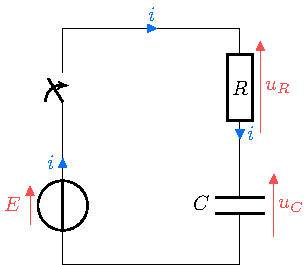
\includegraphics[width=.9\linewidth]{circ_rc-start}
    }%
    \label{fig:circ_rc-start}
    \captionof{figure}{}
  \end{center}
\end{tcb*}

\subsubsection{Équation différentielle du circuit}
\begin{tcb*}[label=demo:eqdiffrc,
  list entry={\lte\thedemo~:~Équa. diff. RC montant}]
  (demo){Équation différentielle RC échelon montant}
	Avec la loi des mailles,
  \vspace{-25pt}
	\psw{%
		\begin{DispWithArrows*}
			u_R + u_C &= E
			\Arrow{$u_R = Ri$\\et $i = C \dv{u_C}{t}$}
			\\\Lra
			RC \dv{u_C}{t} + u_C        & = E
			\\\Lra
			\dv{u_C}{t} + \frac{1}{RC}u_C & = \frac{E}{RC}
		\end{DispWithArrows*}
	}%
	\vspace{-15pt}
\end{tcb*}
\begin{tcb*}[label=prop:eqdiffrc, sidebyside, righthand ratio=.4,
  list entry={\lte\theprop~:~Équa. diff. RC montant}]
  (prop){Équation différentielle RC échelon montant}
	L'équation différentielle de la tension $u_C(t)$ aux bornes d'un condensateur
	dans un circuit RC avec un échelon de tension montant $E$ s'écrit
		\[
      \psw{%
        \boxed{\dv{u_C}{t} + \frac{1}{\tau}u_C = \frac{E}{\tau}}
      }%
      \qav
      \psw{%
        \boxed{\tau = RC}
      }%
		\]
	\tcblower
	C'est une équation différentielle linéaire du premier ordre à
	coefficients et second membre constants, de condition initiale
	\psw{%
		\[
			\boxed{u_C(0^-) = u_C(0^+) = 0}
		\]
	}%
\end{tcb*}

\begin{tcb}(appl)<lftt>{Dimension de $RC$}
	Montrer, par analyse dimensionnelle, que $RC$ est homogène à un temps.
	\tcblower
	\begin{isd}[sidebyside align=top]
		\tcbsubtitle{\fatbox{Méthode 1}}
		\psw{%
			On a $[RC] = \si{\Omega.F}$. Or,
			\begin{align*}
				[q] = [Cu] & \Lra \si{C} = \si{F.V}
				\\
				           & \Lra \si{F} = \si{C.V^{-1}}
				\\
				           & \Lra \si{F} = \si{A.s.V^{-1}}
				\\
        \beforetext{de plus,}
				[u] = [Ri] & \Lra \si{V} = \si{\Omega.A}
				\\
				           & \Lra \si{\Omega} = \si{V.A^{-1}}
				\\
        \beforetext{Ainsi,}
				[RC]         & = \si{\Omega.F}
				\\\Lra
				[RC]         & = \si{V.A^{-1}.A.s.V^{-1}}
				\\\Lra
				\Aboxed{[RC] & = \si{s}}
				\qed
			\end{align*}
		}%
    \vspace{-30pt}
		\tcblower
		\tcbsubtitle{\fatbox{Méthode 2}}
		\psw{%
			Une équation physique étant homogène, comme
			\[
				\dv{u_C}{t} + \frac{u_C}{RC} = \frac{E}{RC}
			\]
			alors
			\begin{align*}
				\left[ \dv{u_C}{t} \right] & = \left[\frac{u_C}{RC}\right]
				\\\Lra
				\frac{[u_C]}{[t]}          & = \frac{[u_C]}{[RC]}
				\\\Lra
				\Aboxed{[RC]               & = [t]}
				\qed
			\end{align*}
		}%
	\end{isd}
\end{tcb}

\subsubsection{Résolution de l'équation différentielle}
\begin{tcb*}[label=impo:eqres,
  list entry={\lte\theror~:~Résolution equa.\ diff.\ ordre 1}]
  (ror){Résolution équation différentielle coefficients constants}
	Pour résoudre une équation différentielle linéaire à
	coefficients constants et second membre constant, de la forme
	$\DS \dv{y}{t} + \frac{1}{\tau}y = k$~:
	\begin{enumerate}[label=\sqenumi]
		\item On écrit l'\textbf{équation homogène} associée à
		      l'équation différentielle obtenue.
		\item On écrit la \textbf{forme générale de la solution de
			      l'équation homogène}.
		\item On recherche une \textbf{solution particulière
			      constante de l'équation générale}, de la forme $y_p(t) =
			      \lambda$.
		\item On écrit la \textbf{solution générale}, somme de la
		      solution particulière et de la forme générale.
		\item On détermine la constante à l'aide des
		      \textbf{conditions initiales}.
	\end{enumerate}
\end{tcb*}

\begin{tcb*}[label=demo:rcsolu, breakable](demo){Tension RC série montant}
	\begin{enumerate}[label=\sqenumi]
		\item L'équation homogène est~:
		      \psw{%
		      \[
			      \dv{u_{C,h}}{t} + \frac{1}{\tau}u_{C,h} = 0
		      \]
		      }%
		      \vspace{-15pt}
		\item La forme générale de la solution pour cette équation est~:
		      \psw{%
			      \[
				      u_{C,h}(t) = K\exp\left( -\frac{t}{\tau} \right)
			      \]
		      }%
		      \vspace{-15pt}
		\item Une solution particulière avec $u_{C,p}(t) = \lambda$ donne
		      \psw{%
			      \[
				      0 + \frac{\lambda}{\tau} = \frac{E}{\tau}
			      \]
			      Donc $u_{C,p}(t) = E$ est \textbf{une} solution de l'équation
			      différentielle.
		      }%
		\item La solution générale est donc
		      \psw{%
			      \[
				      u_C(t) = E + K\exp \left( - \frac{t}{\tau} \right)
			      \]
		      }%
		      \vspace{-15pt}
		\item Les conditions initiales donnent ici
		      \[
			      \psw{u_C(t=0) = 0}
			      \qqet
			      \psw{u_C(0) = K + E \Ra K=-E}
		      \]
	\end{enumerate}
\end{tcb*}
\begin{tcb*}[label=prop:ucsolu, sidebyside, righthand ratio=.3](prop)
  {Tension RC montant}
	La solution de l'équation différentielle de la tension $u_C(t)$
	d'un circuit RC soumis à un échelon de tension $E$ avec
	$u_C(0) = 0$ est
	\psw{%
		\[
			\boxed{u_C(t) = E\left(1-\exp\left(-\frac{t}{\tau}\right)\right)}
		\]
	}%
  et $u_C(t)$ est continue.
	\vspace{-15pt}
	\tcblower
	\begin{center}
		\sswitch{%
			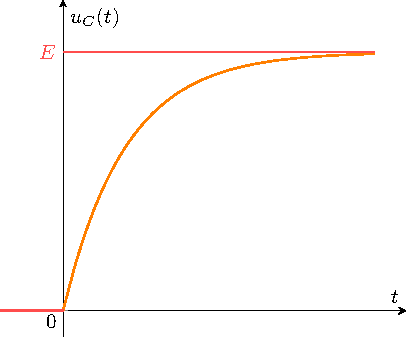
\includegraphics[width=\linewidth, draft=true]{carac_rc}
		}{%
			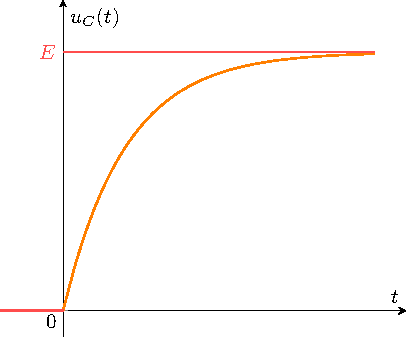
\includegraphics[width=\linewidth]{carac_rc}
		}%
		\captionof{figure}{}
	\end{center}
\end{tcb*}

\subsubsection{Constante de temps, régime transitoire}
Quand $t \ra +\infty$, $u_C(t) = E$. On est alors en \textbf{régime permanent}~:
$u_C(t)$ ne varie plus. La vitesse à laquelle ce régime est atteint dépend de la
valeur de $\tau$ la constante de temps.
  \begin{tcb*}[label=impl:déterm, sidebyside, righthand ratio=.4]
    (impl){Détermination $\tau$ RC montant}
    % Avec la courbe $u_C(t)$, on remarque que~:
    \begin{enumerate}
      \item \psw{%
              $u_C(\tau) = E \left( 1-e^{-1} \right) \approx
                \num{0.632}\times E$
            \smallbreak
            Donc on trouve $\tau$ en lisant l'abscisse telle que $u_C(\tau) =
              \num{0.632}\times E$.
            }%
      \item En $t=0$, l'équation différentielle donne
            \psw{%
              \begin{gather*}
                \dv{u_C}{t}\/ (0) + \underbracket[1pt]{\frac{u_C(0)}{\tau}}_{=0}
                = \frac{E}{\tau}
                \\\Lra
                y_0'(t) = \frac{E}{\tau}
                \Ra 
                \boxed{y_0(t) = E\frac{t}{\tau}}
              \end{gather*}
            }%
            La tangente à la courbe en 0 coupe donc l'asymptote en $\boxed{t =
            \tau}$.
    \end{enumerate}
    \tcblower
    \sswitch{%
      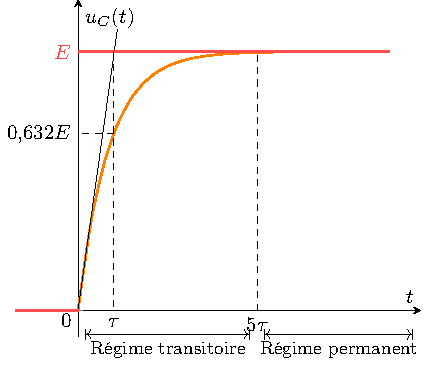
\includegraphics[width=\linewidth, draft=true]{carac_rc-tau}
    }{%
      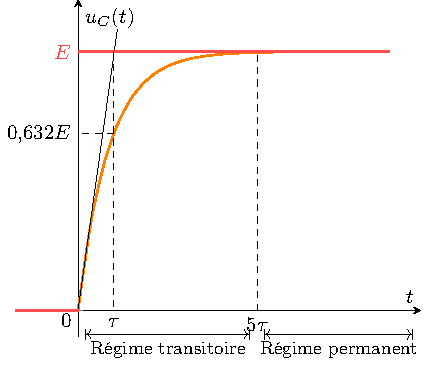
\includegraphics[width=\linewidth]{carac_rc-tau}
    }%
    \captionof{figure}{}
  \end{tcb*}
% On distingue alors deux zones sur la courbe, approximativement séparées~: le
% régime \textit{transitoire} et le régime \textit{permanent}.
\begin{tcb*}(defi){Temps de réponse}
  Le \textbf{temps de réponse} d'un circuit d'ordre 1 est le temps à partir
  duquel on peut considérer la consigne de tension ou de courant atteinte,
  c'est-à-dire qu'on est en \textbf{régime permanent}.
  \smallbreak
  Pour cela, on se fixe un \textbf{seuil arbitraire} à partir duquel on
  considère le régime permanent atteint. 
\end{tcb*}

\begin{tcb*}(demo){Temps de réponse RC montant}
Dans ce cours, on prendra $99\%$. On cherche donc $t_{99}$ tel que $u(t_{99}) =
\num{0.99}E$~:
  \psw{%
    \begin{DispWithArrows*}
      u_C(t_{99}) &= \num{0.99}E
      \Arrow{solution de $u_C$}
      \\\Lra
      E\left(1-\exp(-\frac{t_{99}}{\tau})\right) &= \num{0.99}E
      \CArrow{$\mdiv E$}
      \\\Lra
      1 - \exp\left( -\frac{t_{99}}{\tau} \right) &= \num{0.99}
      \Arrow{on isole l'exp}
      \\\Lra
      \exp\left( -\frac{t_{99}}{\tau} \right) &= \num{0.01}
      \CArrow{$\ln (~)$}
      \\\Lra
      -\frac{t_{99}}{\tau} &= \ln (\num{0.01}) = -\ln (100)
      \Arrow{on isole $t_{99}$}
      \\\Lra
      \Aboxed{t_{99} &= \tau \ln (100)}
    \end{DispWithArrows*}
  }%
  \vspace{-15pt}
\end{tcb*}

\begin{tcb*}(prop){Temps de réponse RC montant}
	\leftcenters{Ainsi,}
	{\psw{\fbox{le temps de réponse à 99\% est à \num{4.6}$\tau$}}}
\end{tcb*}

\subsubsection{Évolution de l'intensité}
Qu'advient-il de l'intensité dans un circuit RC~? On peut le déterminer de deux
manières~:
\begin{tcb*}[label=demo:irc-charge, sidebyside,
  fontupper=\small, fontlower=\small]
  (demo){Intensité RC montant}
  \tcbsubtitle{\fatbox{\textbf{Caractéristique de C}}}
  \psw{%
    \begin{DispWithArrows*}[fleqn, mathindent=-10pt, groups]
      i(t)             & = C\DS \dv{u_C}{t}
      \qav
      u_C(t) = E(1-\exr^{-t/\tau})
      \\\Ra
      i(t) & = CE \left(
      0 - \left(-\frac{1}{\tau} \right)
      \exp \left(- \frac{t}{\tau} \right)
      \right)
      \Arrow{$\tau = RC$}
      \\\Lra
      \Aboxed{i(t) &= \frac{E}{R}\exp \left(-\frac{t}{\tau} \right)}
    \end{DispWithArrows*}
  }%
  \tcblower
  \tcbsubtitle{\fatbox{\textbf{Loi des mailles}}}
  \psw{%
    \begin{DispWithArrows*}[fleqn, mathindent=-10pt, groups]
      Ri &= E-u_C
      \qav
      u_C(t) = E(1-\exr^{-t/\tau})
      \\\Lra
      Ri(t) &= \cancel{E-E}+E \exp(-\frac{t}{\tau})
      \CArrow{$\mdiv R$}
      \\\Lra
      \Aboxed{i(t) &= \frac{E}{R}\exp \left(-\frac{t}{\tau} \right)}
    \end{DispWithArrows*}
  }%
\end{tcb*}
\begin{tcb*}[label=prop:irc-charge, sidebyside, righthand ratio=.3]
  (prop){Intensité RC montant}
	L'intensité dans un circuit RC en charge s'exprime par
	\psw{%
		\[
			\boxed{i(t) = \frac{E}{R}\exp \left(-\frac{t}{\tau} \right)}
		\]
	}%
  et est discontinue.
	\tcblower
	\begin{center}
		\sswitch{%
			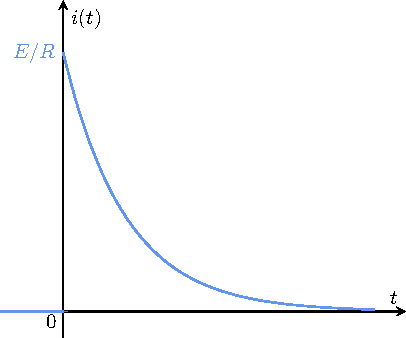
\includegraphics[width=\linewidth, draft=true]{carac_rcI}
		}{%
			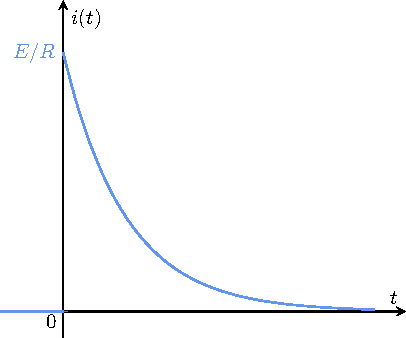
\includegraphics[width=\linewidth]{carac_rcI}
		}%
		\captionof{figure}{}
	\end{center}
\end{tcb*}

\subsubsection{Bilan de puissance}

En électrocinétique, les puissances sont le produit d'une tension et d'une
intensité. Or, par construction la loi des mailles est une relation entre les
tensions du circuit~; ainsi

\begin{tcb*}[fontupper=\Large, bld, cnt](ror){Bilan de puissance en élec.}
	On effectue un bilan de puissance en écrivant la loi des mailles multipliée
	par $i$.
\end{tcb*}
\begin{tcb*}[label=demo:rcpuiss-charge](demo){Bilan de puissances RC montant}
	\vspace{-15pt}
	\psw{%
		\begin{DispWithArrows*}
			u_C + Ri &= E
			\CArrow{$\times i$}
			\\\Lra
			u_C\,i + Ri^{2} &= Ei
			\Arrow{RCT pour C~: $i = C \dv{u_C}{t}$}
			\\\Lra
			u_C\,C \dv{u_C}{t} + Ri^{2} &= Ei
			\Arrow{$f \times f' = \left( \frac{1}{2}f^{2} \right)'$}
			\\\Lra
			\underbracket[1pt]{\dv{t} \left( \frac{1}{2}Cu_C{}^{2} \right)}
			_{\dv{\Ec_C}{t}} +
			\underbracket[1pt]{\vphantom{\dv{t} \left( \frac{1}{2}Cu_C{}^{2} \right)}
				Ri^{2}}_{\Pc_J}
			&=
			\underbracket[1pt]{\vphantom{\dv{t} \left( \frac{1}{2}Cu_C{}^{2} \right)}
				Ei}_{\Pc_G}
		\end{DispWithArrows*}
	}%
	\vspace{-15pt}
\end{tcb*}
\begin{tcb*}[label=prop:rcpuiss-charge](prop){Bilan de puissances RC montant}
	Dans un circuit RC en charge, on a le bilan de puissances
	\psw{%
		\[
			\boxed{\Pc_G = \Pc_C + \Pc_J}
		\]
	}%
	\vspace{-15pt}
	\begin{itemize}[leftmargin=50pt]
		\olditem[$\Pc_G = Ei$] : \psw{%
				la puissance fournie par le générateur~;
			}%
		\olditem[$\Pc_C = \dv{\Ec_C}{t}$] : \psw{%
				la puissance reçue par le condensateur~;
			}%
		\olditem[$\Pc_J = Ri^{2}$] : \psw{%
				la puissance dissipée par effet \textsc{Joule} dans la
				résistance.
			}%
	\end{itemize}
\end{tcb*}

\subsubsection{Bilan d'énergie}
On peut étudier énergétiquement cette évolution en intégrant la puissance
délivrée sur le temps d'utilisation.
% En effet, comme vu précédemment, $i(t)$
% tend vers $0$ en $+\infty$, donc la puissance finale sera nulle et l'énergie
% finie.
\begin{tcb*}[label=demo:rcenerg-charge, breakable]
  (demo){Bilan d'énergie RC montant}
	L'énergie fournie par le générateur sur toute la charge est
	\psw{%
		\begin{DispWithArrows*}[groups]
			\Ec_G &= \int_{0}^{+\infty} \Pc_G \dd t
			\Arrow{$\Pc_G = Ei$}
			\\
			&= \int_{0}^{+\infty} Ei(t) \dd t
			\Arrow{$i(t) = E/R \exr^{-t/\tau}$}
			\\
			&=
			\frac{E^2}{R} \left[
				-\tau \exp \left(-\frac{t}{\tau} \right)
				\right]_0^{+\infty}
			\\
			&=
			\frac{E^{2}}{R}
			\left(
			-\tau \underbracket[1pt]{\exp\left(-\frac{\infty}{\tau}\right)}_{=0}
			- \left( -\tau
				\xunderbracket{\exp(0)}_{=1}
				\right)
			\right)
			\\\Lra
			\Ec_G &= \tau \frac{E^2}{R}
			\Arrow{$\tau = RC$}
			\\\Lra
			\Aboxed{\Ec_G &= CE^2}
		\end{DispWithArrows*}
	}%
  \psw{%
	Or, l'énergie stockée dans le condensateur (Pt.E2.13) est
		\[
			\Ec_C = \frac{1}{2}CE^2
  \qdc
			\Ec_J = \frac{1}{2}CE^2
		\]
	}%
	\vspace{-15pt}
\end{tcb*}
\begin{tcb*}[label=prop:rcenerg-charge, sidebyside]
  (prop){Bilan d'énergie RC montant}
	Pendant la totalité de la charge, l'énergie du générateur est
	\psw{%
		\[\boxed{\Ec_G = CE^2}\]
	}%
  \vspace{-15pt}
  \tcblower
	Elle se répartit équitablement entre le condensateur et la résistance~:
	\psw{%
		\[\boxed{\Ec_C = \frac{1}{2} CE^2 = \Ec_J}\]
	}%
	\vspace{-15pt}
\end{tcb*}

\subsection{Circuit RC série~: décharge}
\subsubsection{Présentation}
\begin{tcb*}[sidebyside, righthand ratio=.30](defi){Circuit RC en décharge}
  \begin{itemize}
    \item Il est constitué d'un générateur idéal de tension en série avec une
          résistance et un condensateur idéal.
    \item \textbf{On suppose le condensateur initialement chargé}~: $u_C(0^-) =
            E$.
    \item À $t=0$, on coupe le générateur.
  \end{itemize}
  On dit que le système est \textbf{en régime libre} et soumis à un
  \textbf{échelon de tension descendant}.
\tcblower
  \begin{center}
    \sswitch{%
      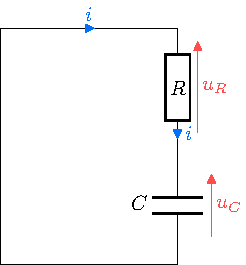
\includegraphics[width=.9\linewidth, draft=true]{circ_rc-decharge}
    }{%
      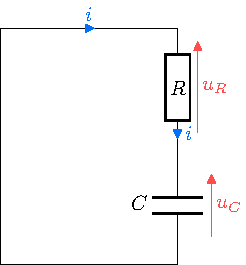
\includegraphics[width=.9\linewidth]{circ_rc-decharge}
    }%
    \label{fig:circ_rc-decharge}
    \captionof{figure}{}
  \end{center}
\end{tcb*}

\subsubsection{Équation différentielle du circuit}
	\begin{tcb*}[label=prop:eqdiffrc, sidebyside,
  list entry={\lte\theprop~:~Équa. diff. RC descendant}]
  (prop){Équation différentielle RC échelon descendant}
		L'équation différentielle de la tension $u_C(t)$ aux bornes d'un
		condensateur dans un circuit RC en décharge
			\[
		\psw{%
        \boxed{\dv{u_C}{t} + \frac{1}{\tau}u_C = 0}
		}%
    \qav
    \psw{%
      \boxed{\tau = RC}
    }%
      \]
		\tcblower
		C'est une équation différentielle linéaire du premier ordre à
		coefficients constants sans second membre, de condition initiale
		\psw{%
			\[ \boxed{u_C(0^-) = u_C(0^+) = E}\]
		}%
	\end{tcb*}
	\begin{tcb*}[label=demo:eqdiffrc,
  list entry={\lte\thedemo~:~Équa. diff. RC descendant}]
  (demo){Équation différentielle RC échelon decendant}
		Avec la loi des mailles,
    \vspace{-25pt}
		\psw{%
			\begin{DispWithArrows*}
				u_R + u_C &= 0
				\Arrow{$u_R = Ri$\\et $i = C \dv{u_C}{t}$}
				\\\Lra
				RC \dv{u_C}{t} + u_C        & = 0
				\\\Lra
				\dv{u_C}{t} + \frac{1}{RC}u_C & = 0
			\end{DispWithArrows*}
		}%
	\end{tcb*}

\subsubsection{Résolution de l'équation différentielle}
	\begin{tcb*}[label=prop:ucsolu](prop){Tension RC descendant}
		La solution de l'équation différentielle de la tension $u_C(t)$
		d'un circuit RC en décharge avec $u_C(0) = E$ est \textbf{continue}, et~:
		\psw{%
			\[\boxed{u_C(t) = E\exp\left(-\frac{t}{\tau}\right)}\]
		}%
	\end{tcb*}
	\begin{tcb*}[label=demo:rcsolu](demo){Tension RC descendant}
		L'équation étant déjà homogène, on écrit la forme générale~:
		\psw{%
			\[u_C(t) = K\exp\left( -\frac{t}{\tau} \right)\]
		}%
		et on trouve $K$ avec la condition initiale~:
		\[
			\psw{u_C(0) = E}
			\qqet
			\psw{u_C(0) = K \Ra K=E}
		\]
	\end{tcb*}

\subsubsection{Représentation graphique, constante de temps et transitoire}
	\begin{tcb}[label=impl:déterm, sidebyside, righthand ratio=.4]
    (impl){Détermination $\tau$ RC descendant}
		\begin{enumerate}
			\item \psw{%
				      $u_C(\tau) = E e^{-1} \approx \num{0.368}\times E$
			      \smallbreak
			      Donc on trouve $\tau$ en lisant l'abscisse telle que $u_C(\tau) =
				      \num{0.368}\times E$.
			      }%
			\item En $t=0$, l'équation différentielle donne
			      \psw{%
				      \begin{gather*}
					      \dv{u_C}{t}\/ (0) + \overbracket[1pt]{\frac{u_C(0)}{RC}}^{=E} = 0
                \\\Lra
                y_0'(t) = -\frac{E}{\tau}
                \Ra 
                \boxed{y_0(t) = -E \frac{t}{\tau}}
				      \end{gather*}
			      }%
			      La tangente à la courbe en 0 coupe donc l'asymptote en $t = \tau$.
		\end{enumerate}
    \tcblower
		\sswitch{%
			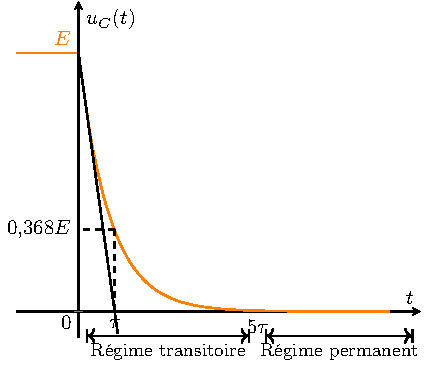
\includegraphics[width=\linewidth, draft=true]{carac_rc-tau_decharge}
		}{%
			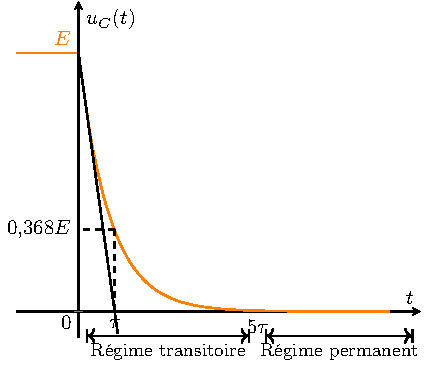
\includegraphics[width=\linewidth]{carac_rc-tau_decharge}
		}%
		\captionof{figure}{}
	\end{tcb}
\begin{tcb*}(demo){Temps de réponse RC descendant}
Comme précédemment, avec $t_{99}$ tel que $u_C(t_{99}) = \num{0.01}E$~:
  \psw{%
    \begin{DispWithArrows*}
      u_C(t_{99}) &= \num{0.01}E
      \Arrow{solution de $u_C$}
      \\\Lra
      E\exp(-\frac{t_{99}}{\tau}) &= \num{0.01}E
      \CArrow{$\mdiv E$}
      \\\Lra
      \exp\left( -\frac{t_{99}}{\tau} \right) &= \num{0.01}
      \CArrow{$\ln (~)$}
      \\\Lra
      -\frac{t_{99}}{\tau} &= \ln (\num{0.01}) = -\ln (100)
      \Arrow{on isole $t_{99}$}
      \\\Lra
      \Aboxed{t_{99} &= \tau \ln (100)}
    \end{DispWithArrows*}
  }%
  \vspace{-15pt}
\end{tcb*}
\begin{tcb*}(prop){Temps de réponse RC descendant}
	\leftcenters{Ainsi,}
	{\psw{\fbox{le temps de réponse à 99\% est à \num{4.6}$\tau$}}}
\end{tcb*}

\subsubsection{Évolution de l'intensité}
\begin{tcb*}[label=demo:irc-charge, sidebyside](demo){Intensité RC décharge}
  \tcbsubtitle{\fatbox{\textbf{Caractéristique de C}}}
  \psw{%
    \begin{DispWithArrows*}[fleqn, mathindent=1pt, groups]
      i(t)             & = C\DS \dv{u_C}{t}
      \qav
      u_C(t) = E\exr^{-t/\tau}
      \\\Ra
      i(t) & = - \frac{CE}{\tau} \exp \left(- \frac{t}{\tau} \right)
      \Arrow{$\tau = RC$}
      \\\Lra
      \Aboxed{i(t) &= -\frac{E}{R}\exp \left(-\frac{t}{\tau} \right)}
    \end{DispWithArrows*}
  }%
  \tcblower
  \tcbsubtitle{\fatbox{\textbf{Loi des mailles}}}
  \psw{%
    \begin{DispWithArrows*}[fleqn, mathindent=1pt]
      Ri &= -u_C
      \Arrow{$u_C(t) = E\exr^{-t/\tau}$}
      \\\Lra
      Ri(t) &= -E \exp(-\frac{t}{\tau})
      \CArrow{$\mdiv R$}
      \\\Lra
      \Aboxed{i(t) &= -\frac{E}{R}\exp \left(-\frac{t}{\tau} \right)}
    \end{DispWithArrows*}
  }%
\end{tcb*}
\begin{tcb*}[label=prop:irc-charge, sidebyside, righthand ratio=.3]
  (prop){Intensité RC décharge}
	L'intensité dans un circuit RC en décharge s'exprime par
	\psw{%
		\[
			\boxed{i(t) = -\frac{E}{R}\exp \left(-\frac{t}{\tau} \right)}
		\]
	}%
  et est discontinue.
	\tcblower
	\begin{center}
		\sswitch{%
			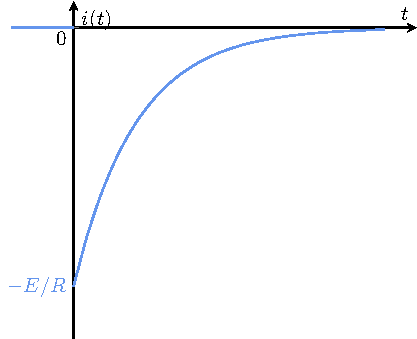
\includegraphics[width=\linewidth, draft=true]{carac_rcI-decharge}
		}{%
			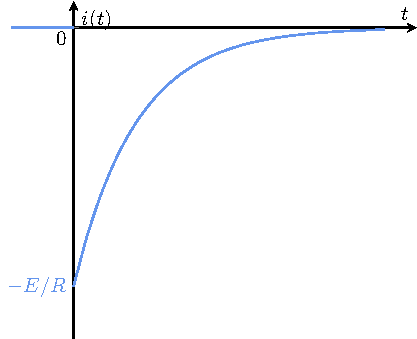
\includegraphics[width=\linewidth]{carac_rcI-decharge}
		}%
		\captionof{figure}{}
	\end{center}
\end{tcb*}

\begin{tcb*}(impo){Conditions initiales}
  \textbf{Attention}, lorsqu'on étudie un circuit charge-décharge, il faut
  \textbf{étudier les conditions initiales en $\boxed{t \neq 0}$}.
\end{tcb*}

\subsection{Méthode pour les circuits à plusieurs mailles}
% En général, les circuits étudiés sont constitués de plus d'une maille. Pour les
% résoudre, on procède comme suit~:
\begin{tcb*}[breakable](ror){Méthode avec plusieurs mailles}
	\begin{enumerate}[label=\sqenumi]
		\item Écrire les différentes lois du circuit (LdN, LdM, Ld$\Omega$, RCT…)~;
		\item Écrire les lois des mailles~;
		\item Isoler la grandeur dont on veut l'équation différentielle en éliminant
		      les autres~;
		\item Mettre l'équation sous forme canonique~:
		      \[
			      \dv{f}{t} + \frac{f}{\tau} = \frac{F}{\tau}
		      \]
		      et identifier $F$ et $\tau$~;
		\item Établir les conditions initiales avec l'énoncé et la continuité de la
		      tension pour $C$~;
		\item Résoudre l'équation différentielle.
	\end{enumerate}
\end{tcb*}

\section{Bobine et circuit RL}
\subsection{Circuit RL série~: échelon montant}
\subsubsection{Présentation}
\begin{tcb*}[sidebyside, righthand ratio=.30](defi){Circuit RC en charge}
  \begin{itemize}
    \item Il est constitué d'un générateur idéal de tension en série avec une
          résistance et une bobine idéals.
    \item \textbf{On suppose l'interrupteur initialement ouvert}.
    \item À $t=0$, on ferme l'interrupteur.
  \end{itemize}
\tcblower
  \begin{center}
    \sswitch{%
      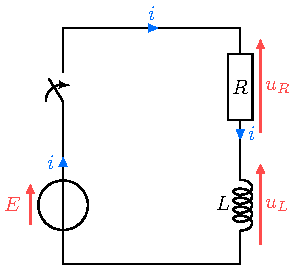
\includegraphics[width=.9\linewidth, draft=true]{circ_rl-start}
    }{%
      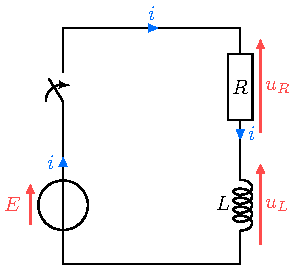
\includegraphics[width=.9\linewidth]{circ_rl-start}
    }%
    \label{fig:circ_rl-start}
    \captionof{figure}{}
  \end{center}
\end{tcb*}

\subsubsection{Équation différentielle du circuit}
% On cherche à connaître l'intensité traversant la bobine à partir du moment où
% l'on ferme l'interrupteur, soit à $t \geq 0$.
\begin{tcb}[label=demo:eqdiffrl,
  list entry={\lte\thedemo~:~Équa. diff. RL montant}]
  (demo){Équation différentielle RL échelon montant}
	Avec la loi des mailles,
  \vspace{-25pt}
	\psw{%
		\begin{DispWithArrows*}
			u_L + u_R &= E
			\Arrow{$u_R = Ri$\\et $u_L = L \dv{i}{t}$}
			\\\Lra
			L \dv{i}{t} + Ri        & = E
			\\\Lra
			\dv{i}{t} + \frac{R}{L}i & = \frac{E}{L}
		\end{DispWithArrows*}
	}%
	\vspace{-15pt}
\end{tcb}
\begin{tcb*}[label=prop:eqdifflc, sidebyside, righthand ratio=.4,
  list entry={\lte\theprop~:~Équa. diff. RL montant}]
  (prop){Équation différentielle RL échelon montant}
	L'équation différentielle du courant $i(t)$ aux bornes d'une bobine
	dans un circuit RL avec un échelon de tension montant $E$ s'écrit
		\[
	\psw{%
			\boxed{\dv{i}{t} + \frac{1}{\tau}i = \frac{1}{\tau}\frac{E}{R}}
	}%
  \qav
  \psw{%
    \boxed{\tau = \frac{L}{R}}
  }%
		\]
	\tcblower
	C'est une équation différentielle linéaire du premier ordre à
	coefficients et second membre constants, de condition initiale
	\psw{%
		\[
			\boxed{i(0^-) = i(0^+) = 0}
		\]
	}%
\end{tcb*}

% \begin{tcb}(rema)<lftt>{Unité de $L/R$}
% 	On peut de même démontrer l'unité de $L/R$ par analyse dimensionnelle.
% \end{tcb}

\subsubsection{Résolution de l'équation différentielle}
\begin{tcb*}[label=demo:rlsolu, breakable](demo){Intensité RL série montant}
	\begin{enumerate}[label=\sqenumi]
		\item L'équation homogène est~:
		      \psw{%
			      \[
				      \dv{i_h}{t} + \frac{1}{\tau}i_h = 0
			      \]
		      }%
		      \vspace{-15pt}
		\item La forme générale de la solution pour cette équation est~:
		      \psw{%
			      \[
				      i_h(t) = K\exp\left( -\frac{t}{\tau} \right)
			      \]
		      }%
		      \vspace{-15pt}
		\item Une solution particulière avec $i_p(t) = \lambda$ donne
		      \psw{%
			      \[
				      0 + \frac{\lambda}{\tau} = \frac{1}{\tau}\frac{E}{R}
			      \]
			      Donc $i_p(t) = \frac{E}{R}$ est \textbf{une} solution de l'équation
			      différentielle.
		      }%
		\item La solution générale est donc
		      \psw{%
			      \[
				      i(t) = \frac{E}{R} + K\exp \left( - \frac{t}{\tau} \right)
			      \]
		      }%
		      \vspace{-15pt}
		\item Les conditions initiales donnent ici
		      \[
			      \psw{i(t=0) = 0}
			      \qqet
			      \psw{i(0) = K + \frac{E}{R} \Ra K=-\frac{E}{R}}
		      \]
	\end{enumerate}
\end{tcb*}
\begin{tcb*}[label=prop:isolu, sidebyside, righthand ratio=.3](prop)
  {Intensité RL montant}
	La solution de l'équation différentielle du courant $i(t)$ d'un circuit RL
	soumis à un échelon de tension $E$ avec $i(0) = 0$ est
	\psw{%
		\[
			\boxed{i(t) = \frac{E}{R}\left(1-\exp\left(-\frac{t}{\tau}\right)\right)}
		\]
	}%
  et $i(t)$ est continue.
	\vspace{-15pt}
	\tcblower
	\begin{center}
		\sswitch{%
			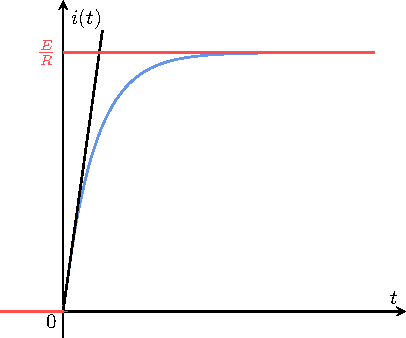
\includegraphics[width=\linewidth, draft=true]{carac_rl}
		}{%
			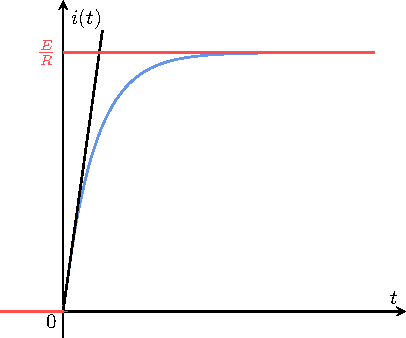
\includegraphics[width=\linewidth]{carac_rl}
		}%
		\captionof{figure}{}
	\end{center}
\end{tcb*}

\subsubsection{Constante de temps, régime transitoire}
  \begin{tcb*}[label=impl:déterm, sidebyside, righthand ratio=.4]
    (impl){Détermination $\tau$ RL montant}
    % Avec la courbe $i(t)$, on remarque que~:
    \begin{enumerate}
      \item \psw{%
              $i(\tau) = \frac{E}{R} \left( 1-e^{-1} \right) \approx
                \num{0.632}\times E/R$
            \smallbreak
            Donc on trouve $\tau$ en lisant l'abscisse telle que $u_C(\tau) =
              \num{0.632}\times E$.
            }%
      \item En $t=0$, l'équation différentielle donne
            \psw{%
              \begin{gather*}
                \dv{i}{t}\/ (0) + \underbracket[1pt]{\frac{i(0)}{\tau}}_{=0}
                = \frac{1}{\tau}\frac{E}{R}
                \\\Lra
                y_0'(t) = \frac{E}{R\tau}
                \Ra 
                y_0(t) = \frac{E}{R} \frac{t}{\tau}
              \end{gather*}
            }%
            La tangente à la courbe en 0 coupe donc l'asymptote en $\boxed{t =
            \tau}$.
    \end{enumerate}
    \tcblower
    \sswitch{%
      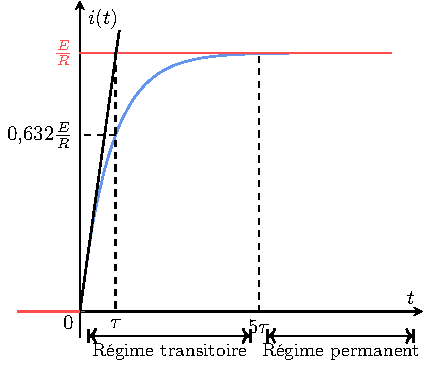
\includegraphics[width=\linewidth, draft=true]{carac_rl-tau}
    }{%
      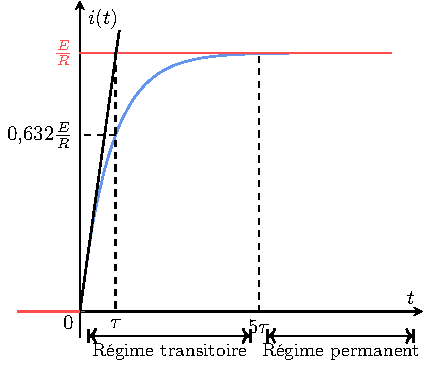
\includegraphics[width=\linewidth]{carac_rl-tau}
    }%
    \captionof{figure}{}
  \end{tcb*}

Comme précédemment, avec $t_{99}$ tel que $i(t_{99}) = \num{0.99}\frac{E}{R}$,
on trouve $t_{99} = \num{4.6}\tau$.
\begin{tcb}(prop){Temps de réponse RL montant}
	\leftcenters{Ainsi,}
	{\psw{\fbox{le temps de réponse à 99\% est à \num{4.6}$\tau$}}}
\end{tcb}

\subsubsection{Évolution de la tension}
\begin{tcb*}[label=demo:url-charge, sidebyside,
  fontupper=\small, fontlower=\small]
  (demo){Tension RL montant}
  \tcbsubtitle{\fatbox{\textbf{Caractéristique de L}}}
  \psw{%
    \begin{DispWithArrows*}[fleqn, mathindent=-10pt, groups]
      u_L(t)             & = L \dv{i}{t}
      \qav
      i(t) = \frac{E}{R}(1-\exr^{-t/\tau})
      \\\Ra
      u_L(t) & = \frac{LE}{R} \left(
      0 - \left(-\frac{1}{\tau} \right)
      \exp \left(- \frac{t}{\tau} \right)
      \right)
      \Arrow{$\tau = \frac{L}{R}$}
      \\\Lra
      \Aboxed{u_L(t) &= E\exp \left(-\frac{t}{\tau} \right)}
    \end{DispWithArrows*}
  }%
  \tcblower
  \tcbsubtitle{\fatbox{\textbf{Loi des mailles}}}
  \psw{%
    \begin{DispWithArrows*}[fleqn, mathindent=-10pt, groups]
      u_L &= E - Ri
      \qav
      i(t) = \frac{E}{R}(1-\exr^{-t/\tau})
      \\\Lra
      u_L(t) &= E -R \frac{E}{R}(1-\exr^{-t/\tau})
      \\\Lra
      \Aboxed{u_L(t) &= E\exp \left(-\frac{t}{\tau} \right)}
    \end{DispWithArrows*}
  }%
\end{tcb*}
\begin{tcb*}[label=prop:url-charge, sidebyside, righthand ratio=.3]
  (prop){Tension RL montant}
	La tension dans un circuit RL en charge s'exprime par
	\psw{%
		\[
			\boxed{u_L(t) = E\exp \left(-\frac{t}{\tau} \right)}
		\]
	}%
  et est discontinue.
	\tcblower
	\begin{center}
		\sswitch{%
			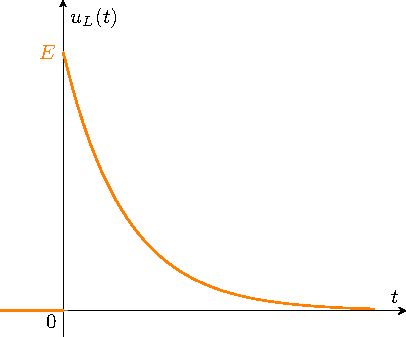
\includegraphics[width=\linewidth, draft=true]{carac_rlU}
		}{%
			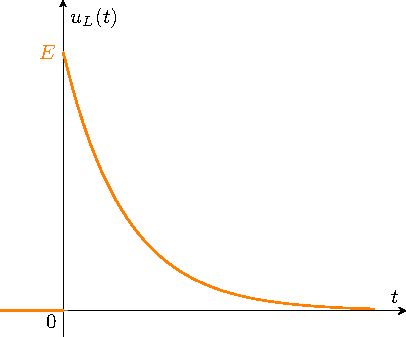
\includegraphics[width=\linewidth]{carac_rlU}
		}%
		\captionof{figure}{}
	\end{center}
\end{tcb*}

\subsubsection{Bilan de puissance}

\begin{tcb*}[label=demo:rlpuiss-charge](demo){Bilan de puissances RL montant}
	\vspace{-15pt}
	\psw{%
		\begin{DispWithArrows*}
			u_L + Ri &= E
			\CArrow{$\times i$}
			\\\Lra
			u_L\,i + Ri^{2} &= Ei
			\Arrow{RCT pour L~: $u_L = L \dv{i}{t}$}
			\\\Lra
			i\,L \dv{i}{t} + Ri^{2} &= Ei
			\Arrow{$f \times f' = \left( \frac{1}{2}f^{2} \right)'$}
			\\\Lra
			\underbracket[1pt]{\dv{t} \left( \frac{1}{2}Li{}^{2} \right)}
			_{\dv{\Ec_L}{t}} +
			\underbracket[1pt]{\vphantom{\dv{t} \left( \frac{1}{2}Li{}^{2} \right)}
				Ri^{2}}_{\Pc_J}
			&=
			\underbracket[1pt]{\vphantom{\dv{t} \left( \frac{1}{2}Li{}^{2} \right)}
				Ei}_{\Pc_G}
		\end{DispWithArrows*}
	}%
	\vspace{-15pt}
\end{tcb*}
\begin{tcb*}[label=prop:rlpuiss-charge](prop){Bilan de puissances RL montant}
	Dans un circuit RL en charge, on a le bilan de puissances
	\psw{%
		\[
			\boxed{\Pc_G = \Pc_L + \Pc_J}
		\]
	}%
	\vspace{-15pt}
	\begin{itemize}[leftmargin=50pt]
		\olditem[$\Pc_G = Ei$] : \psw{%
				la puissance fournie par le générateur~;
			}%
		\olditem[$\Pc_L = \dv{\Ec_L}{t}$] : \psw{%
				la puissance reçue par la bobine~;
			}%
		\olditem[$\Pc_J = Ri^{2}$] : \psw{%
				la puissance dissipée par effet \textsc{Joule} dans la
				résistance.
			}%
	\end{itemize}
\end{tcb*}

\begin{tcb*}[bld, cnt](impo){Bilan d'énergie RL charge}
	Ici la puissance en régime permanent n'est pas nulle~: un courant circule
	toujours dans la résistance qui dissipe $RI^2$. On ne peut intégrer à
	l'infini.
\end{tcb*}

\subsection{Circuit RL série~: décharge}
\subsubsection{Présentation}
\begin{tcb*}[sidebyside, righthand ratio=.30](defi){Circuit RL descendant}
  \begin{itemize}
		\item Il est constitué d'un générateur idéal de tension en série avec une
		      résistance et une bobine idéale.
		\item \textbf{On suppose le courant initialement établi}~: $i(0^-) =
			      \frac{E}{R}$.
		\item À $t=0$, on coupe le générateur.
  \end{itemize}
  On dit que le système est \textbf{en régime libre} et soumis à un
  \textbf{échelon de tension descendant}.
\tcblower
  \begin{center}
    \sswitch{%
      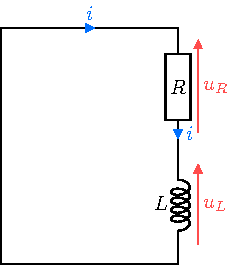
\includegraphics[width=.9\linewidth, draft=true]{circ_rl-decharge}
    }{%
      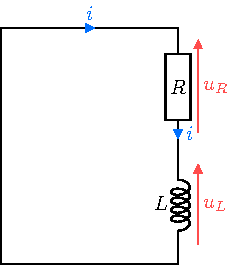
\includegraphics[width=.9\linewidth]{circ_rl-decharge}
    }%
    \label{fig:circ_rl-decharge}
    \captionof{figure}{}
  \end{center}
\end{tcb*}

\subsubsection{Équation différentielle du circuit}
	\begin{tcb*}[label=prop:eqdiffrl, sidebyside,
  list entry={\lte\theprop~:~Équa. diff. RL descendant}]
  (prop){Équation différentielle RL échelon descendant}
		L'équation différentielle du courant $i(t)$ aux bornes d'un
		condensateur dans un circuit RL en décharge
			\[
		\psw{%
        \boxed{\dv{i}{t} + \frac{1}{\tau}i = 0}
		}%
    \qav
    \psw{%
      \boxed{\tau = \frac{L}{R}}
    }%
      \]
		\tcblower
		C'est une équation différentielle linéaire du premier ordre à
		coefficients constants sans second membre, de condition initiale
		\psw{%
			\[ \boxed{i(0^-) = i(0^+) = \frac{E}{R}}\]
		}%
	\end{tcb*}
	\begin{tcb*}[label=demo:eqdiffrl,
  list entry={\lte\thedemo~:~Équa. diff. RL descendant}]
  (demo){Équation différentielle RL échelon decendant}
		Avec la loi des mailles,
		\psw{%
			\begin{DispWithArrows*}
				u_R + u_L &= 0
				\Arrow{$u_R = Ri$\\et $u_L = L \dv{i}{t}$}
				\\\Lra
				L \dv{i}{t} + Ri        & = 0
				\\\Lra
				\dv{i}{t} + \frac{R}{L}i & = 0
			\end{DispWithArrows*}
		}%
	\end{tcb*}

\subsubsection{Résolution de l'équation différentielle}
  \begin{tcb*}[label=prop:rlsoludech](prop){Intensité RL descendant}
    L'intensité $i(t)$ d'un circuit RL en décharge avec $i(0) = \frac{E}{R}$ est
    \textbf{continue}, et~:
		\psw{%
			\[\boxed{i(t) = \frac{E}{R}\exp\left(-\frac{t}{\tau}\right)}\]
		}%
	\end{tcb*}
	\begin{tcb*}[label=demo:rlsoludech](demo){Intensité RL descendant}
		L'équation étant déjà homogène, on écrit la forme générale~:
		\psw{%
			\[i(t) = K\exp\left( -\frac{t}{\tau} \right)\]
		}%
		et on trouve $K$ avec la condition initiale~:
		\[
			\psw{i(0) = \frac{E}{R}}
			\qqet
			\psw{i(0) = K \Ra K=\frac{E}{R}}
		\]
	\end{tcb*}

\subsubsection{Représentation graphique, constante de temps et transitoire}
\begin{tcb*}[label=impl:déterm, sidebyside, righthand ratio=.4]
    (impl){Détermination $\tau$ RL descendant}
		\begin{enumerate}
			\item \psw{%
				      $i(\tau) = \frac{E}{R} e^{-1} \approx
					      \num{0.368}\times \frac{E}{R}$
			      \smallbreak
			      Donc on trouve $\tau$ en lisant l'abscisse telle que $i(\tau) =
				      \num{0.368}\times \frac{E}{R}$.
			      }%
			\item En $t=0$, l'équation différentielle donne
			      \psw{%
				      \begin{gather*}
					      \dv{i}{t}\/ (0) + \overbracket[1pt]{\frac{i(0)}{\tau}}^{=E/R}
					      = 0
                \\\Lra
                y_0'(t) = -\frac{E}{R}
                \Ra 
                \boxed{y_0(t) = -\frac{E}{R} \frac{t}{\tau}}
				      \end{gather*}
			      }%
			      La tangente à la courbe en 0, coupe
			      donc l'asymptote en $\boxed{t = \tau}$.
		\end{enumerate}
    \tcblower
    \sswitch{%
      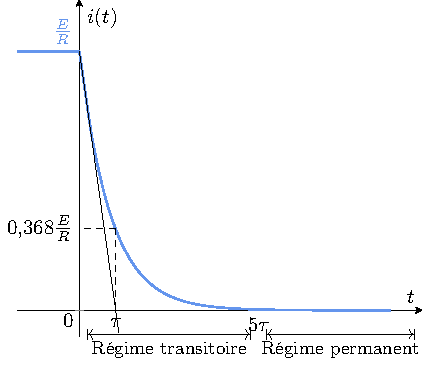
\includegraphics[width=\linewidth, draft=true]{carac_rl-tau_decharge}
    }{%
      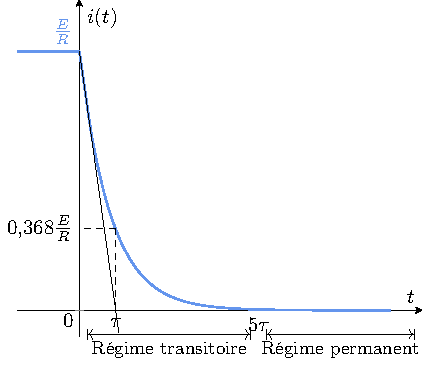
\includegraphics[width=\linewidth]{carac_rl-tau_decharge}
    }%
    \captionof{figure}{}
	\end{tcb*}
Comme précédemment, avec $t_{99}$ tel que $i(t_{99}) = \num{0.01}\frac{E}{R}$,
on trouve $t_{99} = \num{4.6}\tau$.
\begin{tcb*}(prop){Temps de réponse RL descendant}
	\leftcenters{Ainsi,}
	{\psw{\fbox{le temps de réponse à 99\% est à \num{4.6}$\tau$}}}
\end{tcb*}

\subsubsection{Évolution de la tension}
\begin{tcb*}[label=demo:irl-decharge, sidebyside](demo){Tension RL descendant}
  \tcbsubtitle{\fatbox{\textbf{Caractéristique de L}}}
		      \psw{%
            \begin{DispWithArrows*}[fleqn, mathindent=1pt, groups]
				      u_L(t)             & = L \dv{i}{t}
              \qav
				      i(t) = \frac{E}{R}\exr^{-t/\tau}
				      \\\Ra
				      u_L(t) & = -\frac{LE}{R\tau} \exp \left(- \frac{t}{\tau} \right)
				      \Arrow{$\tau = L/R$}
				      \\\Lra
				      \Aboxed{u_L(t) &= -E\exp \left(-\frac{t}{\tau} \right)}
			      \end{DispWithArrows*}
		      }%
  \tcblower
  \tcbsubtitle{\fatbox{\textbf{Loi des mailles}}}
		      \psw{%
            \begin{DispWithArrows*}[fleqn, mathindent=1pt]
				      u_L &= - Ri
				      \Arrow{$i(t) = \frac{E}{R}\exr^{-t/\tau}$}
				      \\\Lra
				      u_L(t) &= -R \frac{E}{R}\exr^{-t/\tau}
				      \\\Lra
				      \Aboxed{u_L(t) &= -E\exp \left(-\frac{t}{\tau} \right)}
			      \end{DispWithArrows*}
		      }%
\end{tcb*}
\begin{tcb*}[label=prop:url-decharge, sidebyside, righthand ratio=.4]
  (prop){Tension RL descendant}
	La tension dans un circuit RL en décharge s'exprime par
	\psw{%
		\[
			\boxed{u_L(t) = -E\exp \left(-\frac{t}{\tau} \right)}
		\]
	}%
  et est discontinue.
	\tcblower
	\begin{center}
		\sswitch{%
			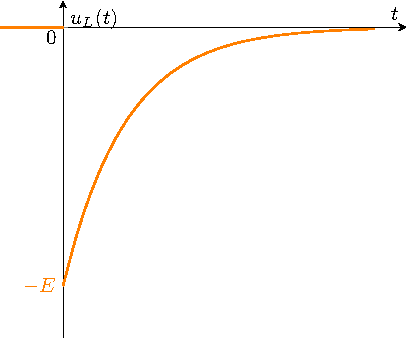
\includegraphics[width=\linewidth, draft=true]{carac_rlU_decharge}
		}{%
			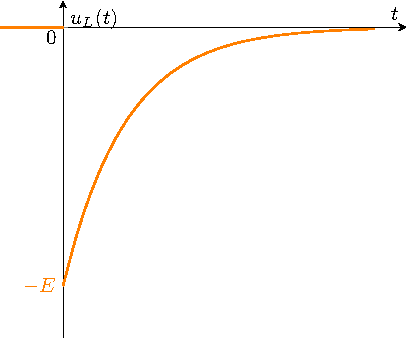
\includegraphics[width=\linewidth]{carac_rlU_decharge}
		}%
		\captionof{figure}{}
	\end{center}
\end{tcb*}

\end{document}
